\section{Introducción}

\begin{frame}
  \frametitle{Muestreo en el dominio de la frecuencia I}

  \begin{columns}[T]
    \begin{column}{7.3cm}

      \begin{itemize}
      \footnotesize
      \item En el tema análisis en frecuencia vimos que la Transformada de Fourier de una Señal Discreta (DTFT) era una función continua en la frecuencia y periódica (con periodo $2\pi$):
      \begin{itemize}
      \footnotesize
      \item  Análisis: \alert{ $X(e^{jw})=\sum_{n=-\infty}^\infty x(n)e^{-jwn}$}
      \item Sintesis:  \alert{$x(n)=\frac{1}{2\pi}\int_{2\pi} X(e^{jw})e^{jwn}$}
      \item Periodicidad: \alert{$X(e^{j(w+2\pi)})=X(e^{j(w+2\pi)})$}
      \end{itemize}
      \visible<2->{
      \item Sin embargo, resulta muy interesante poder representar la señal discreta con \alert{muestras} de su transformada de Fourier:}

      \visible<3->{
      \begin{itemize}
      \footnotesize
      \item Los procesadores digitales de señales trabajan habitualmente con señales discretas (vectores), no con funciones
      \item \alert{El computo de las muestras de la transformada de Fourier es más sencillo que el computo de la función transformada}.

      \end{itemize}}
      \end{itemize}
      \end{column}
      \begin{column}{5cm}
      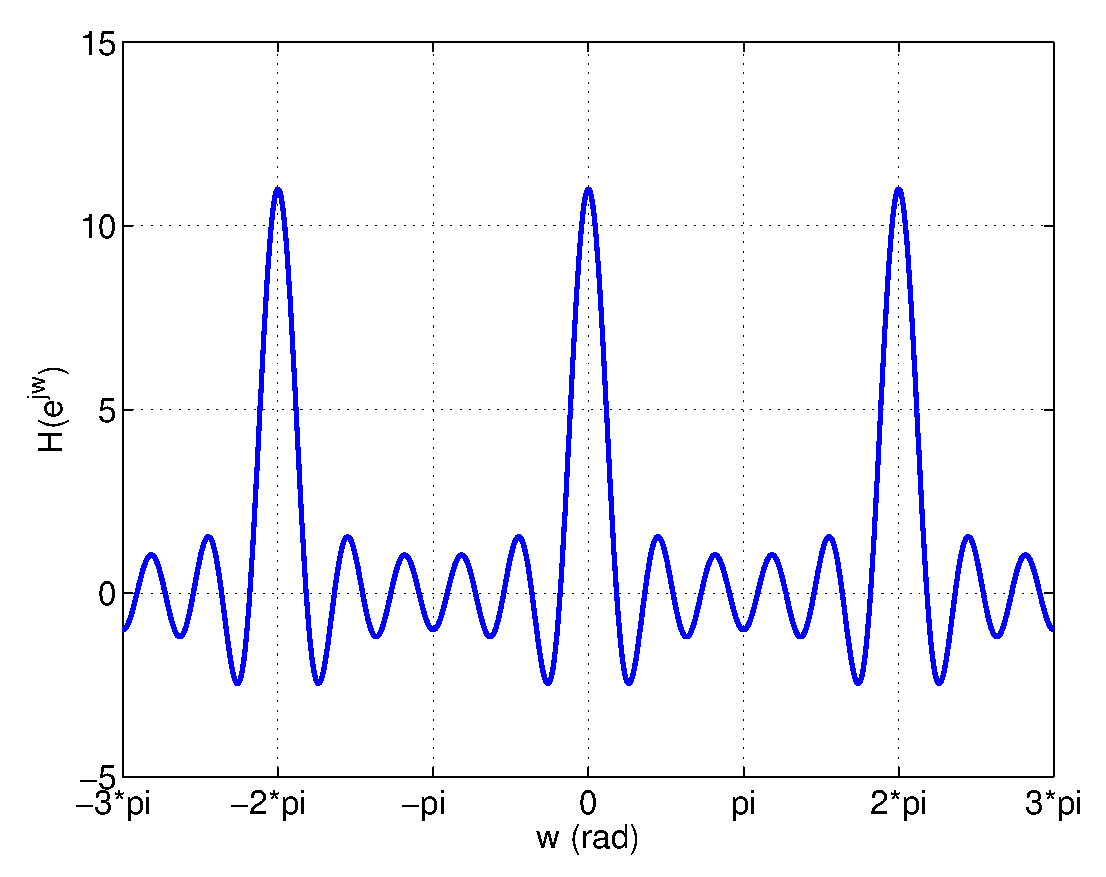
\includegraphics[width=5cm]{./Figures/DFT1.eps}

      \visible<2->{
      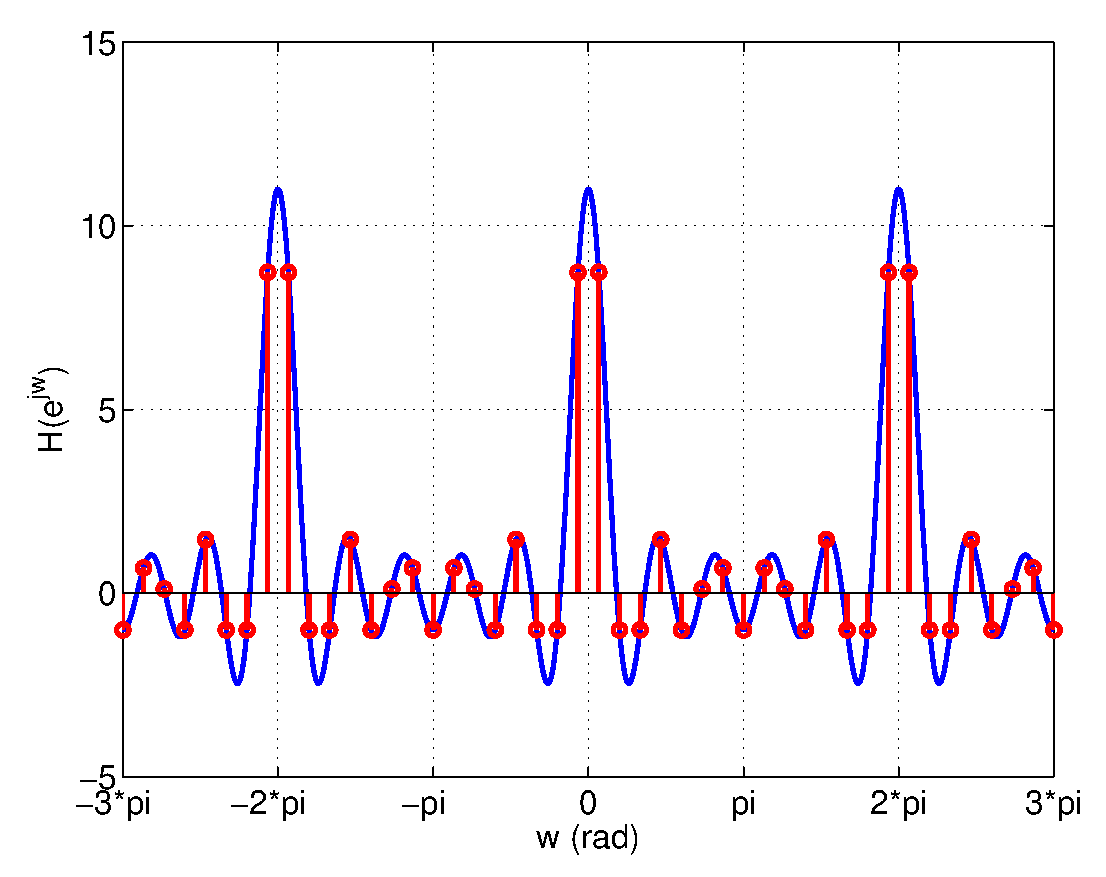
\includegraphics[width=5cm]{./Figures/DFT2.eps}}
    \end{column}
  \end{columns}
\end{frame}

%%%%%%%%%%%%%%%%%%%%%%%%%%%%%%%%%%%%%

\begin{frame}
  \frametitle{Muestreo en el dominio de la frecuencia II}

  \begin{itemize}
    \footnotesize
    \item ¿Como muestreamos de la DTFT ($X(e^{jw})$)?
    \vspace{-0.45cm}
    \begin{columns}[c]
      \hspace{0.9cm}\begin{column}{7cm}
        \begin{itemize}
          \footnotesize
          \visible<2->{\item Para muestrear periódicamente una señal continua $x_a(t)$ en el tiempo, sustituíamos $t=nT$, y hacíamos $x(n)=x_a(nT)$}
          \vspace{-0.1cm}
          \visible<3->{\item Para muestrear la DTFT de la señal discreta, que es continua en $w$, tendremos que hacer $w=k\Delta w$ y $X(k)=X(e^{j\Delta w k})$. }
        \end{itemize}
      \end{column}
      \hspace{-0.8cm}\begin{column}{4cm}
        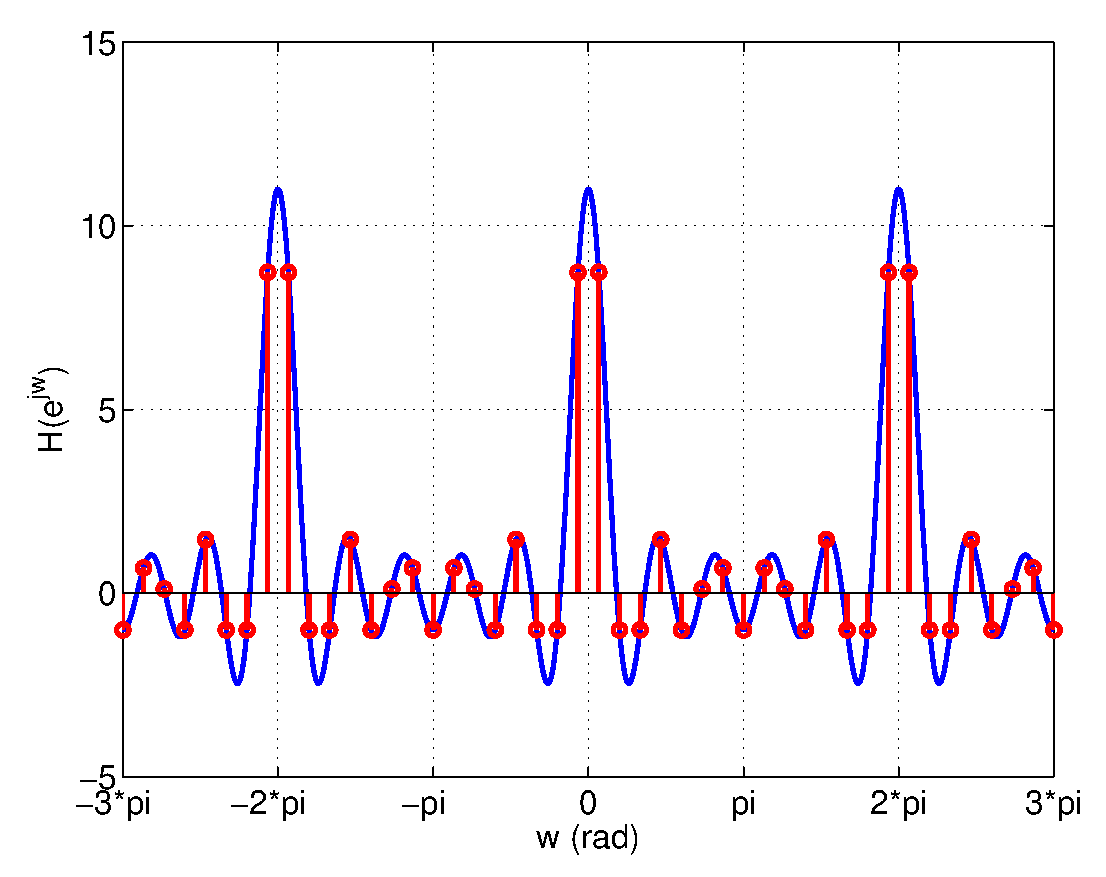
\includegraphics[width=4cm]{./Figures/DFT2.eps}
      \end{column}

    \end{columns}

    \vspace{-0.3cm}

    \begin{itemize}
      \footnotesize
      \visible<4->{\item Para elegir $\Delta w$:}
      \begin{itemize}
        \visible<5->{\item Tenemos en cuenta que $X(e^{jw})$ tiene periodo $2\pi$, y por lo tanto, únicamente es necesario tomar las muestras en el periodo fundamental $[0,2\pi)$}
        \visible<6->{\item Si queremos tomar $N$ muestras equiespaciadas entre $[0,2\pi)$ hacemos de $\Delta w=\frac{2\pi}{N}$}
      \end{itemize}

      \vspace{-0.1cm}

      \visible<7->{
      \item \alert{Las muestras de la DTFT, $X(k)=X(e^{j\frac{2\pi}{N}k})$, reciben el nombre de la Transformada de Fourier Discreta (DFT).} }

      \vspace{0.1cm}

      \visible<8->{
      \scriptsize
      \item La DFT es una señal periódica de periodo N, ya que debido a la periodicidad de la señal $X(e^{jw})$ y el muestreo realizado, cada N muestras la señal se repite. \visible<9->{Ojo: esto no significa que la señal original x(n) tenga que ser periódica. }}
    \end{itemize}

  \end{itemize}
\end{frame}

%%%%%%%%%%%%%%%%%%%%%%%%%%%%%%%%%%%%%%%%%%%%%%%%%%%%%%

\begin{frame}
\frametitle{Reconstrucción de la señal en tiempo discreto I}

  \footnotesize

  \alert{¿Dada la DFT ($N$ muestras de $X(k)$) podemos reconstruir la señal original $x(n)$?}

  \begin{itemize}
    \visible<2->{\item En general no. Pero en algunos casos, si. A continuación analizamos que condiciones se tienen que cumplir, salvo para el caso particular de una señal periódica discreta (relación con la DTFS).}
    \visible<3->{\item Definición de la $X(k)$ a partir de la definición de la $X(e^{jw})$:
    \vspace{-0.1cm}
    $X(e^{jw})=\sum_{n=-\infty}^{\infty} x(n)e^{-jwn}$  $\:\:\: \xrightarrow{w=\frac{2\pi k}{N}}\:\:\: X(k)=\sum_{n=-\infty}^{\infty} x(n)e^{-j\frac{2\pi}{N}kn}$}

    \visible<4->{
    \item Dividimos el sumario sobre n en sumarios de N términos y operamos:

    \scriptsize
    \hspace{-0.7cm}$\alert{X(k)\!=}\!\dots\!+\!\sum_{n=-N}^{-1} x(n)e^{-j\frac{2\pi}{N}\!kn}\!+\!\sum_{n=0}^{N-1} x(n)e^{-j\frac{2\pi}{N}\!kn}\!+\!\sum_{n=N}^{2N-1} x(n)e^{-j\frac{2\pi}{N}\!kn}\!+\!\dots=$}

    \visible<5->{
    $=\!\dots\!+\!\sum_{n=0}^{N-1} \!\!x(n-N)e^{-j\frac{2\pi}{N}\!k(n-N)}\!+\!\sum_{n=0}^{N-1} \!\! x(n)e^{-j\frac{2\pi}{N}\!kn}\!+\!\sum_{n=0}^{N-1} \!\!x(n+N)e^{-j\frac{2\pi}{N}\!k(n+N)}\!+\!\dots$
    }
    \visible<6->{
    $=\!\dots\!+\!\sum_{n=0}^{N-1} \!\!x(n-N)e^{-j\frac{2\pi}{N}\!kn}\!+\!\sum_{n=0}^{N-1} \!\! x(n)e^{-j\frac{2\pi}{N}\!kn}\!+\!\sum_{n=0}^{N-1} \!\!x(n+N)e^{-j\frac{2\pi}{N}\!kn}\!+\!\dots$
    }
    \visible<7->{
    $=\sum_{l=-\infty}^{\infty}\sum_{n=0}^{N-1} x(n-lN) e^{-j\frac{2\pi}{N}\!kn}=\alert{\sum_{n=0}^{N-1}\sum_{l=-\infty}^{\infty} x(n-lN) e^{-j\frac{2\pi}{N}\!kn}}$}

    \visible<8->{
    \footnotesize
    \item Definimos \alert{$x_p(n)=\sum_{l=-\infty}^{\infty} x(n-lN)$}, cuyo valor en un instante $n$ resulta ser el valor que se obtiene sumando los valores de $x(n)$ cada $N$ muestras.}\visible<9->{  Entonces, $\alert{X(k)=\sum_{n=0}^{N-1} x_p(n) e^{-j\frac{2\pi}{N}\!kn}}$.}

    \visible<10->{
    \item Por definición $x_p(n)$ es una función periódica de periodo N:

    $x_p(n+N)=\sum_{l=-\infty}^{\infty} x(n-lN+N) =\sum_{l=-\infty}^{\infty} x(n-lN) =x_p(n)$
    }

  \end{itemize}
\end{frame}

%%%%%%%%%%%%%%%%%%%%%%%%%%%%%%%%%%%%%%%%%%%%%%%%


\begin{frame}
\frametitle{Reconstrucción de la señal en tiempo discreto II}

\vspace{-0.2cm}
\footnotesize
  \begin{itemize}
  \item $\alert{X(k)\!=\!X(e^{j\frac{2\pi}{N}k})\!=\!\sum_{n=0}^{N-1} x_p(n) e^{-j\frac{2\pi}{N}\!kn}}$, transformada de Fourier discreta.
  \item $\alert{x_p(n)\!=\!\sum_{l=-\infty}^{\infty} x(n\!-\!lN)}$, extensión periódica de la señal original.
  \item X(k) y $x_p(n)$ periódicas (periodo N) por construcción.

  \visible<2->{
  \item Como $x_p(n)$ es periódica, podemos representarla a través de su desarrollo en Serie de Fourier (DTFS):}

  \visible<3->{

  \begin{itemize}
  \scriptsize
  \item $x_p(n)=\sum_{k=0}^{N-1} c_k e^{j\frac{2\pi}{N}kn}$}

  \visible<4->{
  \vspace{0.1cm}

  \item $c_k=\frac{1}{N}\sum_{n=0}^{N-1} x_p(n) e^{-j\frac{2\pi}{N}kn}$
  \end{itemize}}
  \visible<5->{
  \item Comparando la expresión de $X(k)$ con la de $c_k$: $c_k=\frac{1}{N}X(k)$.}
  \visible<6->{
  \item Por lo tanto, \alert{$x_p(n)=\frac{1}{N} \sum_{k=0}^{N-1} X(k) e^{j\frac{2\pi}{N}kn}$}.}
  \visible<7->{
  \item La señal periódica $x_p(k)$ se puede reconstruir directamente a partir de la transformada de Fourier discreta ($X(k)$), es decir de las muestras tomadas de la transformada de Fourier en tiempo discreto ($X(e^{jw})$) }
  
  \end{itemize}
  \visible<8->{
  \alert{¿Dada la DFT ($N$ muestras de $X(k)$) podemos reconstruir la señal original $x(n)$?}}
  
  \begin{itemize}
  \visible<9->{
  \item  Si la señal x(n) es de duración finita (distinta de cero sólo durante $L$ instantes sucesivos) y  $L \le  N$, entonces $x_p(n)=x(n)$ y podemos reconstruir la señal original.}
  \item \visible<10->{ Si $L>N$, $x_p(n)\ne x(n)$, se produce aliasing, y la reconstrucción exacta no es posible. }
  \end{itemize}

\end{frame}

%%%%%%%%%%%%%%%%%%%%%%%%%%%%%%%%%%%%


\begin{frame}
\frametitle{Reconstrucción de la señal en tiempo discreto III}

  \footnotesize
  Resumiendo:


  \begin{itemize}
    \item Dada la señal discreta $x(n)$ de duración finita $L$ y su extensión periódica $x_p(n)\!=\!\sum_{l=-\infty}^{\infty} x(n\!-\!lN)$
  \end{itemize}

  \vspace{-0.3cm}
  \vspace{-0.1cm}
  \begin{columns}[c]
    \begin{column}{7.5cm}
      \begin{itemize}
        \item Se tiene que: 

        \begin{itemize}
          \vspace{-0.2cm}
          \footnotesize
          \item ${X(k)\!=\!\sum_{n=0}^{N-1} x_p(n) e^{-j\frac{2\pi}{N}\!kn}}$

          \vspace{0.1cm}

          \item $x_p(n)=\frac{1}{N} \sum_{k=0}^{N-1} X(k) e^{j\frac{2\pi}{N}kn}$
        \end{itemize}
          \visible<2->{
          \item Si $L \le N$:
          \begin{itemize}
          \vspace{-0.4cm}
          \footnotesize
          \item $x_p(n)\!=\!\left\{\!\! \begin{array}{l} x(n), \:\:\:\:\:\:\:\:0\!\le \!n \!\le \!L\!-\!1 \\ 0,  \:\:\:\:\:\:\:\:L\!+\!1\!\le\! n \!\le \!N\!-\!1 \\ x_p(n\!+\!N), \:\:c.c \end{array} \right .$

          \vspace{0.1cm}

          \item $X(k)=\!\sum_{n=0}^{N-1} x(n) e^{-j\frac{2\pi}{N}\!kn}$ 

          \vspace{0.1cm}

          \item $x(n)=\frac{1}{N} \sum_{k=0}^{N-1} X(k) e^{j\frac{2\pi}{N}kn}$

      \end{itemize}}

      \visible<3->{
      \item Si $L>N$ podemos obtener $x_p(n)$ y $X(k)$, pero no $x(n)$, ya que no somos capaces de obtener la $x(n)$ a partir de la $x_p(n)$ o de la $X(k)=X(e^{j\frac{2\pi}{N}k})$.
      }


      \end{itemize}
    \end{column}
    \hspace{-0.9cm}\begin{column}{4cm}
      \visible<1->{
      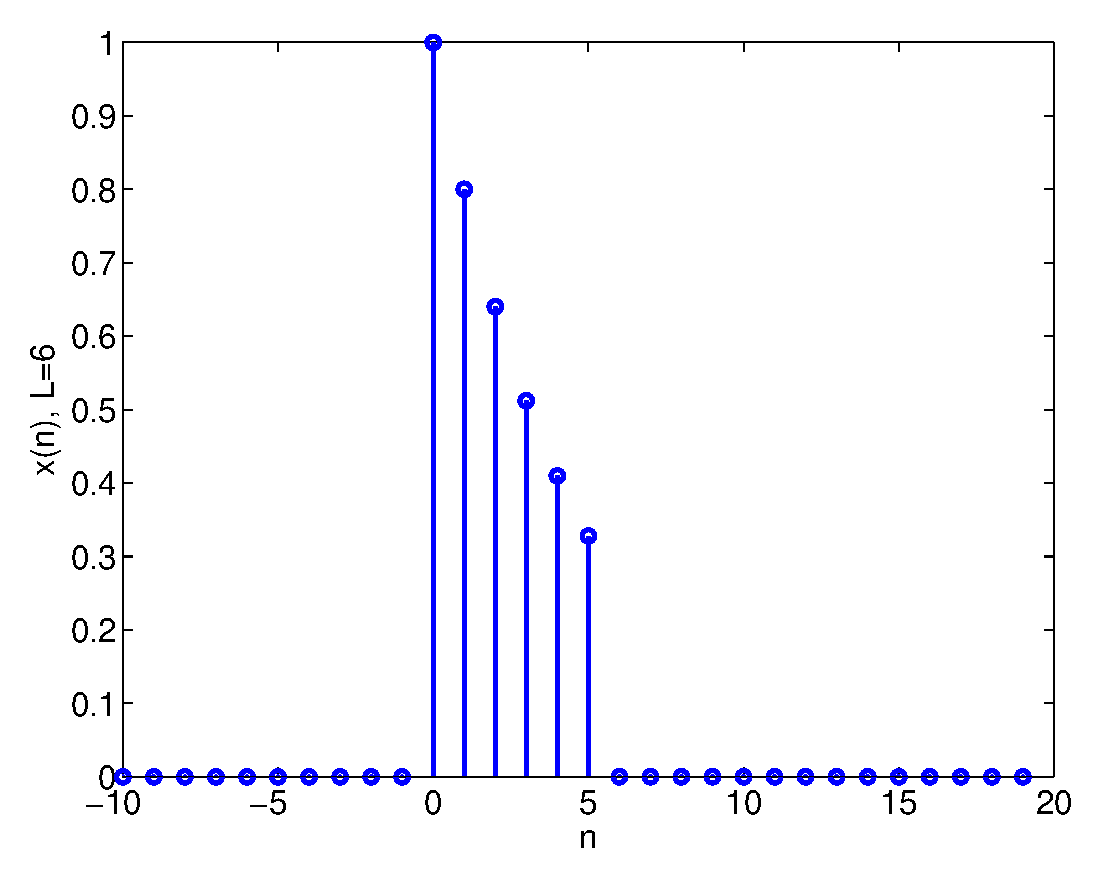
\includegraphics[width=3.5cm,height=2cm]{./Figures/DFTRecXn1.eps}}
      \visible<2->{
      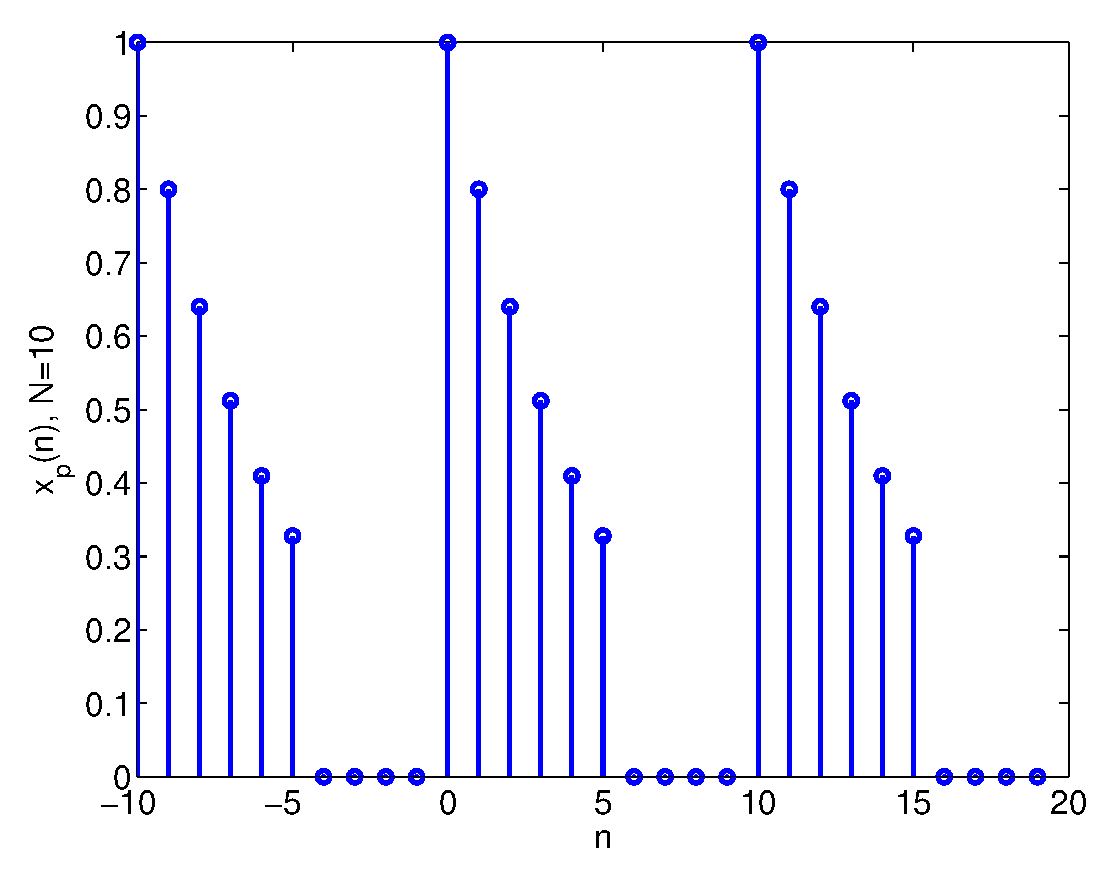
\includegraphics[width=3.5cm,height=2cm]{./Figures/DFTRecXn2.eps}}
      \visible<3->{
      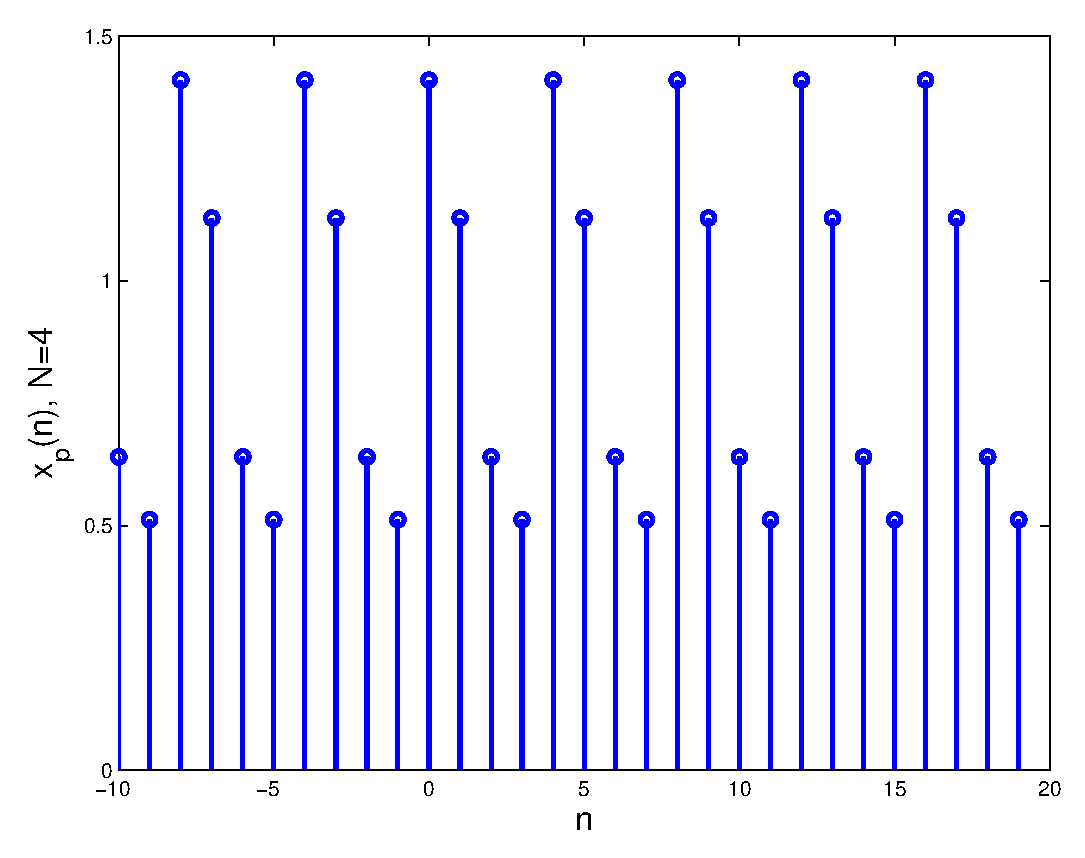
\includegraphics[width=3.5cm,height=2cm]{./Figures/DFTRecXn3.eps}}
    \end{column}
  \end{columns}

\end{frame}

%%%%%%%%%%%%%%%%%%%%%%%%%%%%%%%%%%%%%%%%%%%

\begin{frame}
\frametitle{Reconstrucción de transformada de Fourier I}

  \footnotesize

  \alert{¿Dada la DFT ($N$ muestras de $X(k)$) podemos reconstruir la DTFT ($X(e^{jw})$)?}
 
  \begin{itemize}

    \visible<2->{\item Definición de DTFT: $X(e^{jw})=\sum_{n=-\infty}^{\infty}x(n)e^{-jwn}$}
    \visible<3->{\item Manipulamos la expresión de la DTFT  para buscar la relación entre $X(e^{jw})$ y sus muestras $X(k)$:}
    \begin{itemize}
      \footnotesize
      \visible<4->{\item Como $x(n)$ tiene  longitud finita L, podemos realizar el sumario únicamente sobre los L términos consecutivos de x(n) donde la señal no es cero. Sin embargo, resulta más conveniente hacerlo sobre los N términos, ya que tenemos N muestras en X(k). }
      \visible<5->{
      \item Sustituimos $x(n)=\frac{1}{N} \sum_{k=0}^{N-1} X(k) e^{j\frac{2\pi}{N}kn}$}
      \vspace{0.1cm}
      \visible<6->{\item Reorganizamos sumatorios.}
      \vspace{0.1cm}
      \visible<7->{\item Definimos la función de interpolación $P(e^{jw})=\frac{1}{N}\sum_{n=0}^{N-1}e^{-jwn}$}
    \end{itemize}

    \visible<3->{$\alert{X(e^{jw})}\! =$}\visible<4->{$\sum_{n=0}^{N-1}\!x(n)e^{-jwn}\!=$}\visible<5->{$\sum_{n=0}^{N-1}\!\!\left [\!\frac{1}{N} \sum_{k=0}^{N-1} \!X(k) e^{j\frac{2\pi}{N}kn}\right ] \!\!e^{-jwn}\!=$}
    
    \visible<6->{\hspace{0.9cm} $\!=\!\sum_{k=0}^{N-1} \!X(k) \!\! \left [\frac{1}{N}\sum_{n=0}^{N-1}  e^{j\frac{2\pi}{N}kn} e^{-jwn}\right ]\!=$}

    \visible<6->{\hspace{0.9cm} $\!=\!\sum_{k=0}^{N-1} \!X(k)\! \left [\frac{1}{N}\sum_{n=0}^{N-1}e^{-j(w-\frac{2\pi}{N}k)n}\right ]=$}

    \visible<7->{\hspace{0.9cm}$\alert{=\!\sum_{k=0}^{N-1}\! \!X(k) P(e^{j(w-\frac{2\pi}{N}k)})}$}

  \end{itemize}

\end{frame}

%%%%%%%%%%%%%%%%%%%%%%%%%%%%%%%%%%%%%%%%%%

\begin{frame}
\frametitle{Reconstrucción de transformada de Fourier II}

  \footnotesize

  \alert{¿Dada la DFT ($N$ muestras de $X(k)$) podemos reconstruir la DTFT ($X(e^{jw})$)?}
  
  \footnotesize

  \begin{itemize}
    \item   $X(e^{jw})\! =\!\sum_{k=0}^{N-1}\! \!X(k) P(e^{j(w-\frac{2\pi}{N}k)})$    {\scriptsize \color{gray}(DFT $\leftarrow$ DTFT  para x(n) de longitud finita $L\le N$)\color{black}}
    \item $P(e^{jw})=\frac{1}{N}\sum_{n=0}^{N-1}e^{-jwn}$  {\scriptsize \color{gray}(función de interpolación)\color{black}}

  \end{itemize}

  \begin{columns}[T]
    \begin{column}{6.5cm}
      \begin{itemize}
        \visible<4->{\item Reescribir la expresión de la función de interpolación:}

        \begin{itemize}
          \footnotesize
          \visible<5->{\item $\sum_{n=0}^{N-1} a^n=\frac{1-a^N}{1-a}$}
          \vspace{0.1cm}
          \visible<6->{\item Sacar factor común del numerador y denominador.}
          \vspace{0.1cm}
          \visible<7->{\item Simplificar.}
        \end{itemize}
        \visible<4->{$P(e^{jw})=$}\visible<5->{$\frac{1}{N}\frac {1-e^{-jwN}}{1-e^{-jw}}=$}
        \visible<6->{\hspace{1cm}$=\frac{1}{N}\frac{e^{-j\frac{wN}{2}}}{e^{-j\frac{w}{2}}}\frac {e^{j\frac{wN}{2}}-e^{-j\frac{wN}{2}}}{e^{j\frac{w}{2}}-e^{-j\frac{w}{2}}}= $}
        \visible<7->{\hspace{1cm}$=\frac{sen(\frac{wN}{2})}{N sen(\frac{w}{2}) }e^{-j\frac{w(N-1)}{2}} $}

      \end{itemize}
    \end{column}
    \begin{column}{5cm}
      \visible<2-|handout:1>{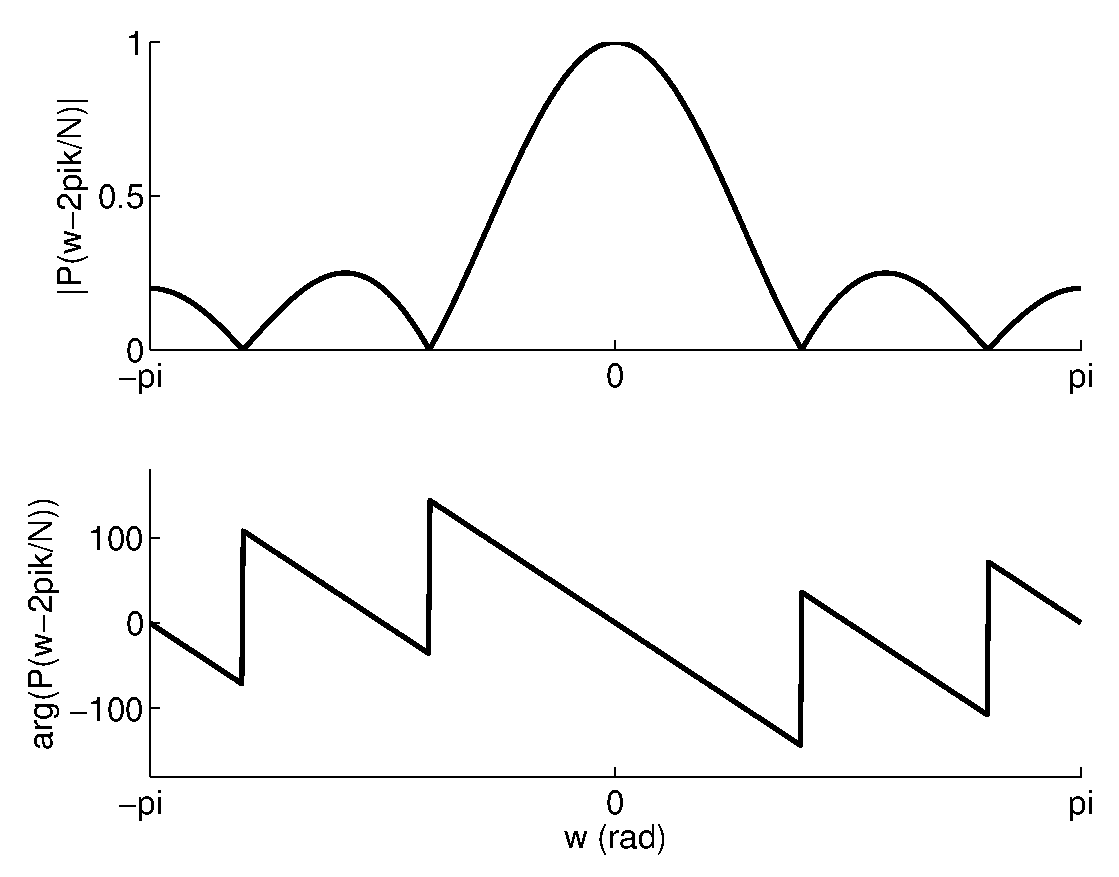
\includegraphics[width=3.5cm]{./Figures/DFTRecHw1.eps}}
      \visible<3-|handout:1>{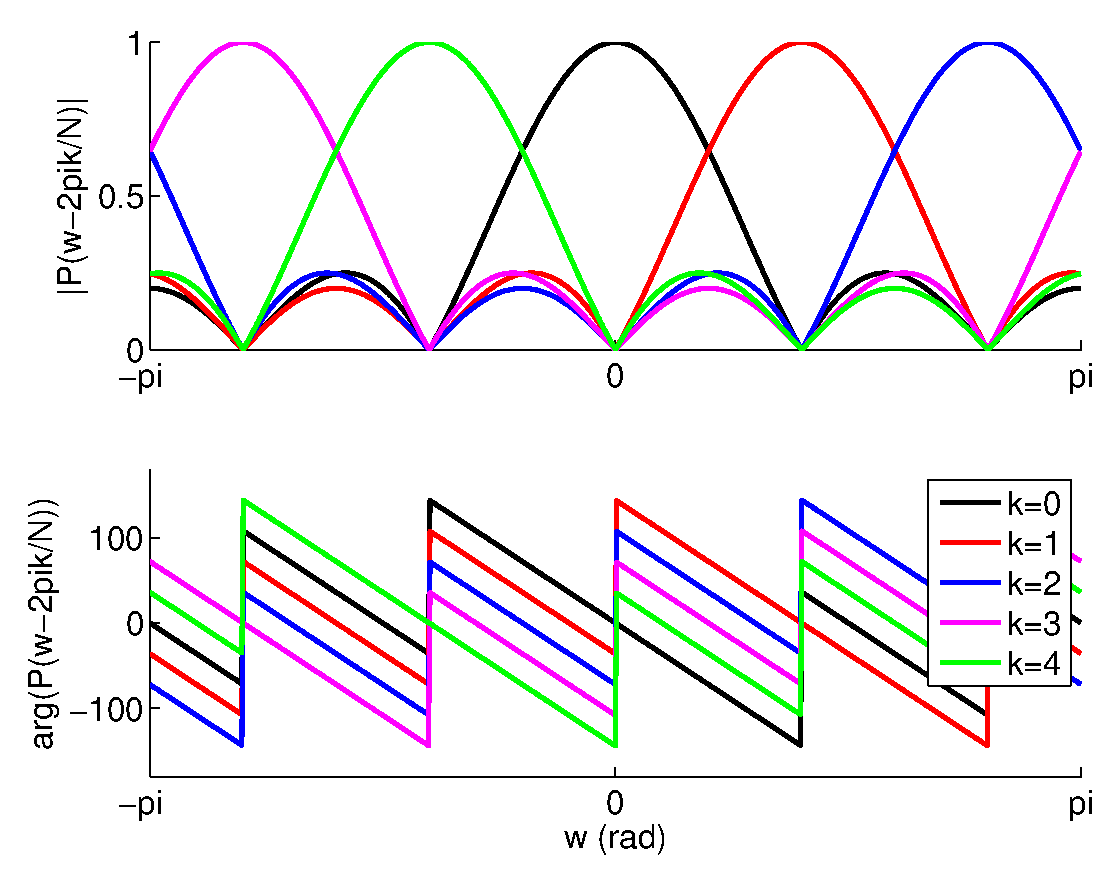
\includegraphics[width=3.5cm]{./Figures/DFTRecHwN.eps}}
    \end{column}
  \end{columns}

\end{frame}
